\documentclass[a4paper,11pt]{article}
\usepackage{graphicx,msc,alltt,float,geometry,tikz,pgf-umlcd,listings,alloy,hyperref}
\setcounter{tocdepth}{2}

\geometry{
	includeheadfoot,
	margin=2.54cm
}

\lstset{ %
  language=alloy,                % the language of the code
  basicstyle=\footnotesize,       % the size of the fonts that are used for the code
  numbers=left,                   % where to put the line-numbers
  numberstyle=\tiny\color{gray},  % the style that is used for the line-numbers
  stepnumber=1,                   % the step between two line-numbers. If it's 1, each line 
                                  % will be numbered
  numbersep=5pt,                  % how far the line-numbers are from the code
}

\begin{document}
	\begin{titlepage}
	\begin{center}

		{\Huge 2IW05 Software Specification\\ Project}\\[0.5cm]
		{\huge Deliverable 1}\\
		\rule{\linewidth}{0.5mm}\\[0.5cm]


		{\Large
		Tim van Dalen\\
		Carl van Dueren den Hollander\\
		Bart Koopmans\\[1cm]
		}

		{\large
		Department of Computer Science\\
		Technical University Eindhoven\\[1cm]
		}

		\begin{abstract}

Abstract

\end{abstract}

		\vfill

		{\large \today}
	\end{center}
\end{titlepage}

	\tableofcontents
	\newpage

	\section{Introduction}
	This document presents a formal specification for the 'Doodle' meeting website for the 2012 fall 2IW05 software specification course.

We will follow a normal iterative approach (with only two iterations for two deliverables) where we will first extract use cases from the informal specification and use them to analyse the informal specification. Then we will use this analysis to form a system design.

\paragraph{}
The goal of this project is to specify a system where people can agree on meeting times. An organizer creates a meeting and specifies dates that are available and people that want to attend the event can vote on times they are available.

When the organizer wants to close the event, all participants receive an email with the final details. We can assume that emails are sent using a reliable third party service which is not part of our system. In this document, we will call this email system "Email" or "Email system".

\paragraph{}
We will describe a basic version of this system and indicate improvements that are out of the scope of this project where we feel they would improve the user experience.

	\newpage
	
	\section{Use cases}
	\label{sec:usecases}
This section describes the use cases of the system. These use cases only cover the basics like creating and managing events and responding to event invites.

A more complete, real-world system could benefit from additions as:
\begin{itemize}
	\item a comment system that allows people to discuss event details.
	\item a richer environment for event organizers that includes a picture gallery.
	\item a notification system on the website.
	\item integration with event features from popular social networks.
	\item more options for inviting people (for instance, allow invitees to invite new people for public events).
	\item allowing closed events to be reopened (and in general a more flexible event system).
\end{itemize}

\subsection{Create meeting schedule}

\begin{description}
	\item[Pre-condition:] User is registered and logged in
	\item[Trigger:] User clicks 'Schedule new event' link
	\item[Guarantee:] A new event is created
	\item[Scenarios]\textbf{:}\\
				\begin{description}
					\item[Main scenarios]\textbf{:}\\
								\begin{enumerate}
									\item The user enters his/her name, the event name and an event description.
									\item The user enters some date/time options.
									\item The user enters email addresses for attendees and a custom message.
									\item The user specifies whether or not the poll should be 'hidden' and voting limitations.
									\item The user submits the event to the system by opening the poll.
									\item The system sends confirmation and invitation emails.
								\end{enumerate}
					\item[Alternatives]\textbf{:}\\
								\begin{itemize}
									\item 2.1 One or more date/time pairs are not valid, the system shows an error message and the user is back at the start of step 2, with all fields already filled in, except for the invalid ones.
								\end{itemize}
				\end{description}
\end{description}


\subsection{Respond to a meeting invitation}

\begin{description}
	\item[Pre-condition:] User has received an invitation email and the meeting poll is open
	\item[Trigger:] User clicks the link in the invitation email
	\item[Guarantee:] The user voted on possible dates
	\item[Scenarios]\textbf{:}\\
				\begin{description}
					\item[Main scenarios]\textbf{:}\\
								\begin{enumerate}
									\item The user confirms that he or she would like to attend the event.
									\item The user votes on date/time options.
									\item The system sends a notification email to the organizer.
									\item The user is able to see the votes of other invitees.
								\end{enumerate}
					\item[Alternatives]\textbf{:}\\
								\begin{itemize}
									%TODO: Not sure if an alternative is really the way to go. I used to have a seperate use case for accepting and declining, but that seemed a bit superfluous.
									\item 1.1 If the user doesn't want to participate in the event, he or she declines the invitation.	The use case is ended
									\item 2.1 If the organizer made any voting restrictions, such as enabling users to only vote once or limiting the number of invitees that can vote on a certain date/time, these are enforced. They will continue to step 3.
									\item 4.1 If the poll was marked 'hidden' by the organizer, the results are not shown. The use case is ended.
								\end{itemize}
				\end{description}
\end{description}

\subsection{Edit a meeting response}

\begin{description}
	\item[Pre-condition:] User has responded to a meeting invitation and the meeting poll is open
	\item[Trigger:] User clicks the link in the invitation email
	\item[Guarantee:] The users can confirm his presence by answering the poll.
	\item[Scenarios]\textbf{:}\\
				\begin{description}
					\item[Main scenarios]\textbf{:}\\
								\begin{enumerate}
									\item The user confirms that he/she would still like to attend the event.
									\item The user votes on date/time options.
									\item The system sends a notification email to the organizer.
									\item The user is able to see the votes of other invitees.
								\end{enumerate}
					\item[Alternatives]\textbf{:}\\
								\begin{itemize}
									\item 1.1 If the user doesn't want to participate anymore, he or she can decide to decline the invitation. The use case is ended
									\item 4.1 If the poll was marked 'hidden' by the organizer, the results are not shown. The use case is ended.
								\end{itemize}
				\end{description}
\end{description}

\subsection{Administrate an event}

\begin{description}
	\item[Pre-condition:] The user is the organizer for this event
	\item[Trigger:] User clicks the link to administrate the event
	\item[Guarantee:] Settings for the event might have changed
	\item[Scenarios]\textbf{:}\\
				\begin{description}
					\item[Main scenarios]\textbf{:}\\
								\begin{enumerate}
									\item The user is presented with an overview of the event.
									\item The user chooses to delete the event, edit the general settings, change the date/time options or view event logs.
								\end{enumerate}
				\end{description}
\end{description}

\subsection{Close an event}

\begin{description}
	\item[Pre-condition:] The user is the organizer for this event
	\item[Trigger:] User clicks the link to administrate the event and then clicks the delete button
	\item[Guarantee:] The event is closed
	\item[Scenarios]\textbf{:}\\
				\begin{description}
					\item[Main scenarios]\textbf{:}\\
								\begin{enumerate}
									\item The system let user confirms his choice.
									\item The user selects the final date/time based on the poll results.
									\item Optionally, the user enters a closing message for the event.
									\item An email containing the optional message and the final date/time is sent to each invitee that confirmed.
									\item The event is closed.
								\end{enumerate}
					\item[Alternatives]\textbf{:}\\
								\begin{itemize}
									\item 1.1 If the user clicks 'no', the closing is cancelled. The use case is ended.
								\end{itemize}
					\item[Design decision:] Wewant to confirm the choice because when the event is deleted there is no way back and it will cancel the whole event.
					
				\end{description}
\end{description}


	\newpage
	
	\section{Analysis}
	This section aims to give a first analysis of the system.

\subsection{High-level entities}
	Figure~\ref{fig:analysis-model} identifies the high-level entities in the system.
	
	\begin{figure}[H]
		\centering
		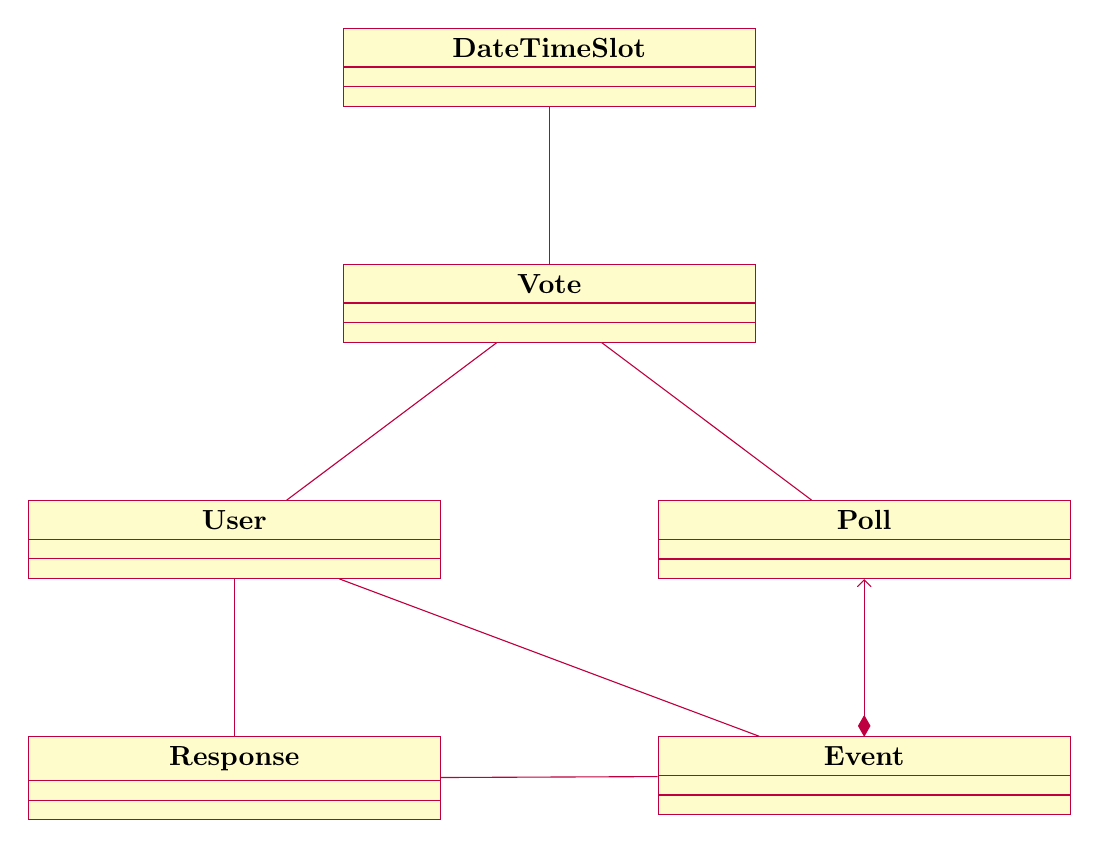
\begin{tikzpicture}
			\begin{class}{User}{0,3}
			\end{class}
		
			\begin{class}{Vote}{4,6}
			\end{class}

			\begin{class}{DateTimeSlot}{4,9}
			\end{class}

			\begin{class}{Poll}{8,3}
			\end{class}

			\begin{class}{Event}{8,0}
			\end{class}

			\begin{class}{Response}{0,0}
			\end{class}

			\association{Response}{}{}{User}{}{}
			\association{Response}{}{}{Event}{}{}
			\association{DateTimeSlot}{}{}{Vote}{}{}
			\association{Vote}{}{}{User}{}{}
			\association{Vote}{}{}{Poll}{}{}
			\association{User}{}{}{Event}{}{}
			\composition{Event}{}{}{Poll}
		\end{tikzpicture}
		\caption{High-level entities in the system}
		\label{fig:analysis-model}
	\end{figure}
	
\subsection{System level sequence diagram}
	%Note: These should be for each use case, with System one entity and entities for the actors
%\begin{figure}[H]
%%\centering
%%\begin{msc}{Use case 1}
%%%\declinst{usr}{User}{}
%%%\declinst{sys}{System}{}
%%%
%%%\mess{Message}{usr}{sys}
%%\end{msc}
%%\caption{One}
%%\label{smsc:one}
%\end{figure}

	\newpage
	
	\section{Design model}
	\subsection{Class diagram}
	\begin{figure}[H]
		\centering
		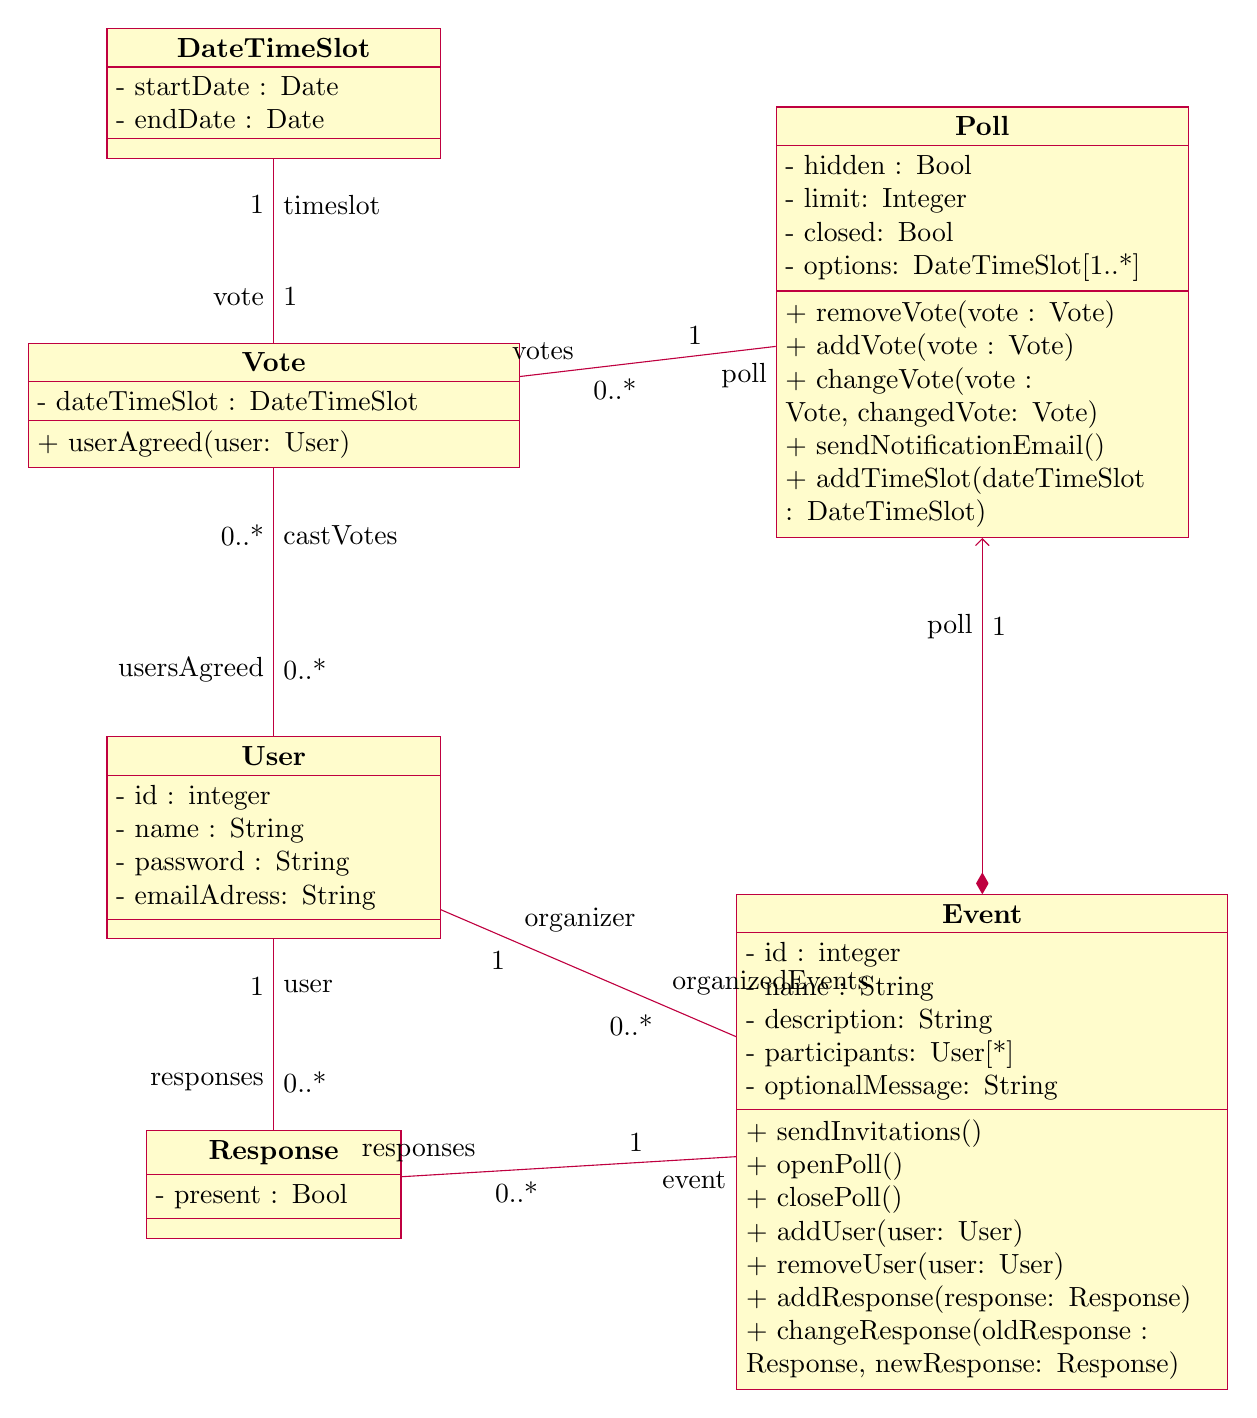
\begin{tikzpicture}
			%Ignore the {x,y} values while working on this, we'll change that later
			\begin{class}[text width=4cm]{User}{0,5}
			\attribute{- id : integer}
			\attribute{- name : String}
			\attribute{- password : String}
			\attribute{- emailAdress: String}
			\end{class}
		
			\begin{class}[text width=6cm]{Vote}{0,10}
			\attribute{- dateTimeSlot : DateTimeSlot }
			\operation{+ userAgreed(user: User)}
			\end{class}

			\begin{class}[text width=4cm]{DateTimeSlot}{0,14}
			\attribute{- startDate : Date}
			\attribute{- endDate : Date}
			\end{class}

			\begin{class}{Poll}{9,13}
			\attribute{- hidden : Bool}
			\attribute{- limit: Integer}
			\attribute{- closed: Bool}
			\attribute{- options: DateTimeSlot[1..*]}
			\operation{+ removeVote(vote : Vote)}
			\operation{+ addVote(vote : Vote)}
			\operation{+ changeVote(vote : Vote, changedVote: Vote)}
			\operation{+ sendNotificationEmail()}
			\operation{+ addTimeSlot(dateTimeSlot : DateTimeSlot)}
			\end{class}

			\begin{class}[text width=6cm]{Event}{9,3}
			\attribute{- id : integer}
			\attribute{- name : String}
			\attribute{- description: String}
			\attribute{- participants: User[*]}
			\attribute{- optionalMessage: String}
			\operation{+ sendInvitations()}
			\operation{+ openPoll()}
			\operation{+ closePoll()}
			\operation{+ addUser(user: User)}
			\operation{+ removeUser(user: User)}		
			\operation{+ addResponse(response: Response)}
			\operation{+ changeResponse(oldResponse : Response, newResponse: Response)}

			\end{class}

			\begin{class}[text width=3cm]{Response}{0,0}
			\attribute{- present : Bool}
			\end{class}


			%Syntax: \aggregation{ClassA}{varOfClassA}{MultofA}{ClassB}{MultofB}{varOfClassB}
			%I'm pretty sure not all are a two-way association
			\association{Response}{responses}{0..*}{User}{1}{user}
			\association{Response}{responses}{0..*}{Event}{1}{event}
			\association{DateTimeSlot}{timeslot}{1}{Vote}{1}{vote}
			\association{Vote}{castVotes}{0..*}{User}{0..*}{usersAgreed}
			\association{Vote}{votes}{0..*}{Poll}{1}{poll}
			\association{User}{organizer}{1}{Event}{organizedEvents}{0..*}
			\composition{Event}{poll}{1}{Poll}
		\end{tikzpicture}
		\caption{High-level entities in the system}
		\label{fig:class-diagram}
	\end{figure}

	For most private attributes we have left out getters and setters because they are implied. For some attributes however, like the responses attribute of Event and the votes attribute of Poll, for which elements can change, we have supplied some getters, setters and changers.

	Classes represent real-world entities as described in section~\ref{sec:analysisdiagram}.

	\emph{Note: We assume there exists a class called \textnormal{Date} that represents a date and a time.}

\subsection{Message Sequence Diagrams}
	\subsubsection{Create meeting schedule}i
		\begin{figure}[H]
			\centering
			\begin{msc}{Create meeting schedule}
				\declinst{org}{User}{Organizer}
				\dummyinst{evt}
				\dummyinst{poll}
				\declinst{email}{Email}{}
				\declinst{inv}{User}{Invitee}

				\create{new}{org}{evt}{Event}{}
				\nextlevel
				\nextlevel
				\create{new}{evt}{poll}{Poll}{}
				\nextlevel

				\mess{setName()}{org}{evt}
				\nextlevel
				\mess{setDescription()}{org}{evt}
				\nextlevel
				\mess{addTimeSlot()}{org}{evt}
				\nextlevel
				\mess{addTimeSlot()}{evt}{poll}
				\nextlevel
				\mess{addTimeSlot()}{org}{evt}
				\nextlevel
				\mess{addTimeSlot()}{evt}{poll}
				\nextlevel
				\nextlevel

				\mess{addUser()}{org}{evt}
				\nextlevel
				\mess{addUser()}{org}{evt}
				\nextlevel
				\nextlevel

				\mess{setHidden()}{org}{evt}
				\nextlevel
				\mess{setHidden()}{evt}{poll}
				\nextlevel
				\nextlevel

				\mess{openPoll()}{org}{evt}
				\nextlevel
				\regionstart{coregion}{evt}
				\nextlevel
				\mess{Send confirmation}{evt}{email}
				\nextlevel
				\mess{Send confirmation}{email}{org}
				\nextlevel
				\mess{sendInvitation()}{evt}{email}
				\nextlevel
				\mess{sendInvitation()}{email}{inv}
				\nextlevel
				\regionend{evt}
				\nextlevel
			\end{msc}
			\caption{Create meeting schedule}
			\label{msc:createmeeting}
		\end{figure}

		The procedure modelled above will be executed once the User, the Organizer of the Event, clicks the link indicating that he or she wants to create a new Event. 
		To do so the User Organizer needs to enter a name, description and possible timeslots. These time slots will be entered into the Poll. After entering this general information the Organizer needs to add other Users to the event, to be invited. All that is left is for the Organizer to choose wether to make the Poll visible to the other users. Now that all options have been set the Organizer needs to open the Poll.
		After all event information has been received, messages will be sent through the Email service to all Users involved. A confirmation message will be sent to the 	Organizer and Invitations will be sent to all invited Users.

	\subsubsection{Respond to meeting invitation}
		\begin{figure}[H]
			\centering
			\begin{msc}{Respond to meeting invitation}
				\declinst{usr}{User}{Invitee}
				\dummyinst{resp}
				\declinst{evt}{Event}{}
				\declinst{poll}{Poll}{}
				\declinst{email}{Email}{}
				\declinst{org}{User}{Organizer}

				\create{new}{usr}{resp}{Response}
				\nextlevel
				\nextlevel
				\nextlevel
				\mess{setPresent()}{usr}{resp}
				\nextlevel
				\nextlevel

				\mess{addResponse(this, response)}{usr}{evt}
				\nextlevel
				\nextlevel

				\mess*{options}{poll}{evt}
				\mess*{Show DateTimeSlot options}{evt}{usr}
				\nextlevel
				\mess{Vote on options}{usr}{evt}
				\mess{Vote}{evt}{poll}
				\nextlevel
				\mess{Notification}{evt}{email}
				\mess{Send notification}{email}{org}
				\nextlevel
				\nextlevel
				
				\mess{Show stats}{evt}{usr}
				\nextlevel
			\end{msc}
			\caption{Respond to meeting invitation}
			\label{msc:respondinvite}
		\end{figure}

		This MSC models a run of the system for the usecase "Respond to meeting invitation", which describes a case where a user receives an invitation to attend an event. In our model, we assume that this can only happen via email, but one could imagine a system where already existing users receive a notification op the homepage of the website.

		The user creates a new Response, containing 'true' for his presence. This Response is added to the Event the user was invited for. The Event reads the options from its Poll and then shows them to the User. The user submits a Vote. The Event saves this in the Poll.
		It then notifies the email service which will send an email to the organizer.
		The Event will then show the statistics (number of votes for each possible DateTimeSlot) to the User.

	\subsubsection{Edit meeting response}
		\begin{figure}[H]
			\centering
			\begin{msc}{Respond to meeting invitation}
				\declinst{usr}{User}{Invitee}
				\declinst{resp}{Repsonse}{}
				\declinst{evt}{Event}{}
				\declinst{poll}{Poll}{}
				\declinst{email}{Email}{}
				\declinst{org}{User}{Organizer}

				\mess{setPresent()}{usr}{resp}
				\nextlevel
				\nextlevel

				\mess{changeResponse(this, response)}{usr}{evt}
				\nextlevel
				\nextlevel

				\mess*{options}{poll}{evt}
				\mess*{Show DateTimeSlot options}{evt}{usr}
				\nextlevel
				\mess*{previous votes}{poll}{evt}
				\mess*{Show previous votes}{evt}{usr}
				\nextlevel
				\mess{Vote on options}{usr}{evt}
				\mess{Vote}{evt}{poll}
				\nextlevel
				\mess{Notification}{evt}{email}
				\mess{Send notification}{email}{org}
				\nextlevel
				\nextlevel
				
				\mess{Show stats}{evt}{usr}
				\nextlevel
			\end{msc}
			\caption{Respond to meeting invitation}
			\label{msc:respondinvite}
		\end{figure}

		This message sequence diagram models the "Edit meeting response" use case. A user can change his present for the event. He can confirm that he is present or he can change it in a later stage when he decide he will not come to the event. When he is present he will vote when the event will be planned. If the votes are not hidden the user can see if the others are present.\\\\
		The first step is when the user set his present, the user decide he is present or not. This will be send to the response class so the response class if the user is coming or not. The user can change this present status anytime ( if the event is not cancelled or closed) then the present status of the corresponding respone will be changed to the desired present status. If the user is present then vote options of the timestamps will be send to the user. The user can also see the votes from other people when the poll is not hidden. After this the user can send his votes. And at least the system returns the stats of the event to the user.

	\subsubsection{Administrate event}
		\begin{figure}[H]
			\centering
			\begin{msc}{Administrate event}
				\declinst{org}{User}{Organizer}
				\declinst{evt}{Event}{}

				\mess{Show event overview}{evt}{org}
				\nextlevel
				\mess{Show options}{evt}{org}
				\nextlevel
				\mess{Change option/delete/view log}{org}{evt}
				\nextlevel
				\mess*{}{evt}{org}
			\end{msc}
			\caption{Administrate event}
			\label{msc:adminevent}
		\end{figure}

		This message sequence chart is a fairly simple one, modelling the behaviour from the "Administrate event" use case, which describes an Event administrator trying to modify a setting of an Event.

		The User first gets an overview of the Event and then is presented with all options, which can then be modified.

	\subsubsection{Close event}
		\begin{figure}[H]
			\centering
			\begin{msc}{Close an event}
				\declinst{org}{User}{Organizer}
				\declinst{evt}{Event}{}
				\declinst{poll}{Poll}{}
				\declinst{email}{Email}{}
				\declinst{inv}{User}{Invitee}

				\mess{Are you sure?}{evt}{org}
				\nextlevel
				\mess{Yes}{org}{evt}
				\nextlevel
				\nextlevel

				\mess{Poll results}{evt}{org}
				\nextlevel
				\mess{Select final DateTimeSlot}{org}{evt}
				\nextlevel
				\mess{Enter optional closing message}{org}{evt}
				\nextlevel
				\mess{Confirm email}{evt}{email}
				\nextlevel
				\mess{setClosed()}{evt}{poll}
				\regionstart{coregion}{email}
				\nextlevel
				\mess{Confirm email}{email}{inv}
				\nextlevel
				\mess{Confirm email}{email}{org}
				\nextlevel
				\regionend{email}
			\end{msc}
			\caption{Close an event}
			\label{msc:closeevent}
		\end{figure}

	\newpage
	
	\section{Formal Specification}
	This section gives a formal specification of our system. Our class diagram has some redundant links in it, which made the specification much harder. When we figured out why some of our predicates were invalid, we didn't have time to change the model anymore, so we tried deep comparing instead of normal comparing.

An example of this is the \texttt{addResponse} predicate. We wanted to specify that the new set of responses was the old set of responses unioned with a singleton containing the new response, but because of the links in Response, User and Event, this was not possible.

\subsection{Sigs}
	\subsubsection{Core module}
		This is our core module. Because of some of the predicates, all sigs have to be in here, except for DateTimeSlot.
	
		\lstinputlisting{alloy/Core.als}
	
	\subsubsection{DateTimeSlot}
	
		\lstinputlisting{alloy/DateTimeSlot.als}
	
\subsection{Facts}
	All facts about the core are in one module, factsCore.
	
	\lstinputlisting{alloy/factsCore.als}
	
\subsection{Preds}
	\subsection{Show the core}
		A trivial predicate to show everything.
		
		\lstinputlisting{alloy/predShowCore.als}
		
	\subsection{Event}
		Some predicates for the Event sig.
		
		\lstinputlisting{alloy/predsEvent.als}
		
	\subsection{Poll}
		Some predicates for the Poll sig.
		
		\lstinputlisting{alloy/predsPoll.als}
		
\subsection{Trace}
	The following images give a trace of our specification.
	
\subsection{Get the specification}
	To download this complete set of files, you can clone our git repository at \texttt{git://github.com/timvdalen/2IW05-project.git}. You can also browse the code online at \url{https://github.com/timvdalen/2IW05-project/tree/master/alloy}.
	\newpage
	
\end{document}
